\chapter{More About Configuring MATSim}
\label{ch:configuring}
% ##################################################################################################################

\hfill \textbf{Author:} Andreas Horni, Kai Nagel

\begin{center} 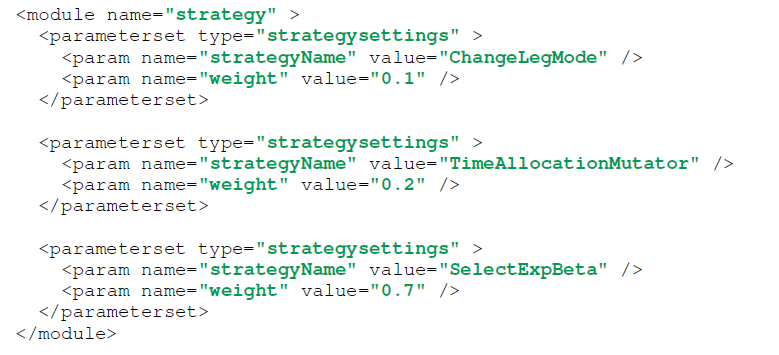
\includegraphics[width=0.3\textwidth, angle=0]{using/figures/strategy.png} \end{center}

% ##################################################################################################################
In this chapter, configurations are described that are exclusively done by the \gls{configfile}. Configurations that require further input data beyond the \gls{configfile} a population and a network are described in Chapter~\ref{ch:modules}.

% ##################################################################################################################
\section{MATSim Data Containers}
\label{sec:using-matsim-containers}

\kai{Eigentlich steht das alles schon in Section \ref{sec:inputdata}.  Ist es wirklich sinnvoll, das zu doppeln?  Oder schreiben wir hier halt die "weiteren" Container rein (dann sollten wir aber einiges weitere von oben hier runter holen).}
\ah{Korrektur begonnen. Tabelle~\ref{tab:modules} Referenzen angepasst und Population wegen \lstinline|ObjectAttributes| nach Extending verfrachtet.}

% ===================================================================================
%\subsection{Network}
%\label{sec:using-network}
%%
%\begin{compactitem}
%\item Invoking the module: By adding the respective configuration file section, the module is invoked automatically.
%\item Configuring: \lstinline|network| config file section
%\item Code: \lstinline|org.matsim.core.network|
%\end{compactitem}

%##################################################################################################################
\section{Global Modules and Global Aspects}
\label{sec:using-globalmodules}
% ===================================================================================
\subsection{Controler}
\label{sec:using-controler}
%
\begin{compactitem}
\item Invoking the module: Run \lstinline|org.matsim.run.Controler|
\item Configuration: \lstinline|controler| configuration file section
%\item Code: \lstinline|org.matsim.core.controler|
\end{compactitem}

The controler is an indispensable module for running \gls{matsim}.

\ah{delete or extend}

% ===================================================================================
\subsection{Global}
\label{sec:global}
\begin{compactitem}
\item Invoking the module: The module is very sparse and only used to transfer some parameters to the simulation. Add a respective config file section.
\item Configuration: \lstinline|global| config file section. Arguably, this section should be merged with the controler section.
%\item Code: \lstinline|org.matsim.core.config.groups.GlobalConfigGroup|
\end{compactitem}

The replanning modules get their information about number of threads from this module. \kai{nicht unter parallel computing?  Wäre meiner Erfahrung nach tatsächlich hilfreich, die paralellen Aspekte zusammenzufassen.}

\ah{\url{https://matsim.atlassian.net/browse/MATSIM-310}} 

% ===================================================================================
\subsection{Parallel Computing}
\label{sec:parallelcomputing}
\begin{compactitem}
\item Invoking the module: Define the number of threads in the \lstinline|qsim| and the \lstinline|parallelEventHandling| section
\item Configuration: \lstinline|parallelEventHandling| and \lstinline|qsim| configuration file section
%\item Code: mainly \lstinline|org.matsim.core.events.ParallelEventsManagerImpl| for parallel event handling. See qsim for parallel mobsim running.
\end{compactitem}

As described in \citet[][]{WaraichEtAl_TechRep_IVT_2009, WaraichEtAl_STRC_2009} the simulation can be substantially speed-up when using multiple threads for the events handling, usually being a bottleneck in \gls{matsim} simulation runs. Amongst others, in the \lstinline|parallelEventHandling| configuration file section, the number of threads to be used can be specified. 
% Clearly, the number of threads should correspond with available processor cores.  \kai{Meine Erfahrung ist eine andere, und je nach Maschine kann man das manchmal überauslasten und manchmal sollte man es eher unterauslasten.}  
According to our experiences the optimal degree of capacity utilization (threads versus cores) is highly machine-dependent.
As mentioned above, the \gls{mobsim} \gls{qsim} is running parallel by default.

Being able to speed-up scenarios might become even more important than today, when additional innovation (choice) dimensions are added with large variability in the parameters rendering ensemble runs necessary. % (see Section~\ref{sec:variability}).

%\ah{Marcel hatte mal Testreihe mit Identifikation der Laufzeit einzelner Module (QSim, Eventshandling etc.) geplant. Nachfragen, ob schon was vorhanden}

% ##################################################################################################################
\section{\protect\glspl{mobsim}}
\label{sec:using-mobsims}
An overview of \gls{matsim} mobility simulations is given in \citet[][]{Dobler_TechRep_IVT_2011}. %See also the presentation of \citet[][]{Rieser_unpub_IVT_2011}.

% ===================================================================================
\subsection{\protect\gls{qsim}}
\label{sec:using-qsim}
\begin{compactitem}
\item Invoking the module: Set the parameter \lstinline|mobsim| of \lstinline|controler| config file section to \lstinline|qsim| provide a \lstinline|qsim| \gls{configfile} section.
\item Configuration: \lstinline|qsim| config section
%\item Code: \lstinline|org.matsim.core.mobsim.qsim|
\end{compactitem}

At the moment, in most applications the queue-based and time-step based \gls{qsim} \citep[][]{Dobler_TechRep_IVT_2011, Dobler_STRC_2010} is used. 
%% It has started as a software branch of \emph{queueSimulation} before supplanting this later simulation. 
Through multiple engines it can be run in parallel. 

% ===================================================================================
\subsection{JDEQSim}
\label{sec:jdeqsim}
\begin{compactitem}
\item Invoking the module: Set the parameter \lstinline|mobsim| of \lstinline|controler| config file section to \lstinline|JDEQSim| provide a \lstinline|jdeqsim| config file section.
\item Configuration: \lstinline|jdeqsim| config file section
\item Code: \lstinline|org.matsim.core.mobsim.jdeqsim|
\end{compactitem}

\gls{jdeqsim} \citep[][]{WaraichEtAl_TechRep_IVT_2009, WaraichEtAl_STRC_2009} was used for project \emph{KTI Frequencies} \citep[][]{BalmerEtAl_ResRep_datapuls_2010}. It is is a \gls{java} reimplementation of \gls{deqsim} \citep[][]{WaraichEtAl_STRC_2009, CharyparEtAl_TRR_2007, CharyparEtAl_TRB_2009} and provides parallel event handling but no parallel simulation \citep[][p.11]{BalmerEtAl_ResRep_datapuls_2010}. Back-propagating gaps are supported. Traffic lights, public transport and within-day replanning are not supported.

%##################################################################################################################
\section{Scoring}
\label{sec:scoring}
\begin{compactitem}
\item Invoking the module: add below section to config file
\item Configuration: \lstinline|planCalcScore| config file section
%\item Code: \lstinline|org.matsim.core.scoring|
\end{compactitem}
%
The parameters related to scoring described in Chapter~\ref{ch:scoring}.

\ah{delete or extend}

%##################################################################################################################
\section{Strategy Modules}
\label{sec:strategymodules}
%\kai{Habe ``strategy'' ans Ende gezogen, weil ein matsim run so auch tatsächlich losgeht: erst mobsim, dann scoring, dann replanning.  Gibt es Argumente für andere Reihenfolgen?} \ah{nein, super Punkt!}
The strategy modules are the basic innovation modules available in \gls{matsim}. We do not call them \emph{choice} modules although they are involved in people's choice making. The choice process, however, is performed over the iterations with an \emph{implicit} choice set and it is not based on explicit probability function drawing. Usually, innovation modules also do no define their own utility function. This is particularly true for random mutation modules, where best response modules such as destination innovation are closer to the standard procedure of choice modeling but still not full-blown choice models. For a detailed discussion of \gls{matsim} in choice modeling context see Chapter~\ref{ch:discretechoice}.

All strategy modules are called by configuring the strategy module in the configuration file as shown in the following example.
%
\begin{lstlisting}
<module name="strategy" >
	<parameterset type="strategysettings" >
		<param name="strategyName" value="ChangeLegMode" />
		<param name="weight" value="0.1" />
	</parameterset>
	
	<parameterset type="strategysettings" >
		<param name="strategyName" value="TimeAllocationMutator" />
		<param name="weight" value="0.2" />
	</parameterset>
	
	<parameterset type="strategysettings" >
		<param name="strategyName" value="SelectExpBeta" />
		<param name="weight" value="0.7" />
	</parameterset>
</module>
\end{lstlisting}
%
Each module is given a weight which determines the probability by which the course of action represented by the module is taken. The weights of the strategy modules are renormalized in case they do not sum to one. In this example, each agent changes his leg mode with probability 0.1, its plan timing with probability 0.2. A strategy module is, in the code, always a combination of a plan selector and zero or more strategy module elements. In the example, the agent chooses a plan from his set of plans according to a logit model with probability 0.7. \ah{sollte man immer noch von proba reden, wo wir sie doch im Code endlich losgeworden sind? Andererseits ist es ja tatsächlich eine proba.}

By specifying the parameter \lstinline|subpopulation|, i.e.,\,\
\begin{lstlisting}
<param name="subpopulation" value="externalAgent"/>
\end{lstlisting}
replanning strategies can be applied to distinct sub-populations.

In older versions of the \gls{configfile} you will find following deprecated configuration using numbered strategy modules.
%
\begin{lstlisting}
<module name="strategy" >
    <param name="ModuleProbability_1" value="0.1" />
    <param name="Module_1" value="ChangeLegMode" />
    <param name="ModuleProbability_2" value="0.2" />
    <param name="Module_2" value="TimeAllocationMutator" />
    <param name="ModuleProbability_3" value="0.7" />
    <param name="Module_3" value="SelectExpBeta" />
</module>
\end{lstlisting}
%
\kai{Hier gibt es eine neue, bessere Syntax.  NB dass wir da gerade noch am ``Verhandeln'' sind!}
\ah{angepasst}
%
By specifying the parameter \lstinline|ModuleSubpopulation_X|, i.e.,\,
\begin{lstlisting}
<param name="ModuleSubpopulation_1" value="externalAgent"/>
\end{lstlisting}
replanning strategies can be applied to distinct sub-populations.

Please note, that combining strategy modules that are \glspl{contribution} such as destination innovation and public transport is not straight forward. Combine them with care and contact the mailing list in case you are unsure.

%Combining different modules is not straight-forward in MATSim. This important topic urgently awaits future analysis. To begin with, here, the combination of the strategy modules with public transport is presented in Table \ref{tab:combination}.
%
%% ----------------------------------
%\createtable%
%{Strategy Module Combination}%
%{Strategy Module Combination}%
%{\label{tab:combination}}%
%{%
  %\begin{tabular}[c]{|c|c|c|}
   %\hline
%\textbf{Innovation Dimension}	& \textbf{Default Strategy} & \textbf{Public Transport}\\
%\hline
%time innovation & TimeAllocationMutator &  TransitTimeAllocationMutator\\
%\hline
%route innovation & ReRoute & ReRoute \\
%\hline
%mode innovation & \multirow{2}{*}{ChangeLegMode} & \multirow{2}{*}{TransitChangeLegMode} \\
%(all legs get same mode) &  &  \\
%\hline
%mode innovation & \multirow{2}{*}{ChangeSingleLegMode} & \multirow{2}{*}{TransitChangeSingleLegMode} \\
%(each leg can have a different mode) &  &  \\
%\hline
%mode innovation & \multirow{2}{*}{SubtourModeChoice} & \multirow{2}{*}{TransitSubtourModeChoice} \\
%(subtour-based) &  &  \\
%\hline
%destination innovation & LocationChoice & LocationChoice \\
%\hline
  %\end{tabular}
%}%
%{}

%\kai{Ich meine, dass es diese Transit Sonderformen gar nicht mehr gibt.  ????}
%\ah{habs mal auskommentiert und die Warnung über Contrib-Kombinationen oben hingeschrieben.} 

% ===================================================================================
\subsection{Time Innovation}
\label{sec:timechoice}
\begin{compactitem}
\item Invoking the module: Time choice is applied by defining its parameters in the configuration file and by adapting the configuration file strategy module as follows
%
\begin{lstlisting}
<module name="strategy" >
    <param name="ModuleProbability_1" value="0.x" />
    <param name="Module_1" value="TimeAllocationMutator" />
    [...]
</module>
\end{lstlisting}
%
\item Configuration: \lstinline|TimeAllocationMutator| config file section
%\item Code: \lstinline|org.matsim.core.replanning.modules.TimeAllocationMutator|
\end{compactitem}

The module shifts activity end times randomly within a configurable range as described by \citet[][]{BalmerEtAl_Timmermans_2005, Raney_PhDThesis_2005, Balmer_unpub_VSP_2004, BalmerEtAl_unpub_EIRASS_2004, BalmerEtAl_unpub_STRC_2004}. A best-reponse approach to time choice is applied by "Planomat" described in Section~\ref{sec:planomat}.

% ===================================================================================
\subsection{Route Innovation}
\label{sec:routechoice}
\begin{compactitem}
\item Invoking the module: Route choice is applied by defining its parameters in the configuration file and by adapting the configuration file strategy module as follows
%
\begin{lstlisting}
<module name="strategy" >
    <param name="ModuleProbability_1" value="0.x" />
    <param name="Module_1" value="ReRoute" />
    [...]
</module>
\end{lstlisting}
%
\item Configuration: \lstinline|planscalcroute| config file section. The routing algorithm needs to be specified in the configuration file controler module
%
\begin{lstlisting}
<module name="controler" >
    <param name="routingAlgorithmType" value="{Dijkstra | FastDijkstra |
    		AStarLandmarks | FastAStarLandmarks}" />
    [...]
</module>
\end{lstlisting}
%\item Code: \lstinline|org.matsim.core.router|
\end{compactitem}
%
\gls{matsim} routing is described by \citet[]{LefebvreBalmer_STRC_2007, LefebvreBalmer_TechRep_IVT_2007}. 

The configuration necessary for public transport is shown in Chapter \ref{ch:pt}.  \kai{Da steht m.E.\ noch nichts in der Richtung.  Aber meiner Erinnerung nach ist auch gar keine Sonderkonfiguration mehr nötig.  Michael Z.?}

\ah{Kann tatsächlich auch keine Sonderkonfiguration (mehr) finden unter \url{http://www.matsim.org/docs/tutorials/transit}. Kann man also wegmachen. Muss zu Config-Param "transitRouter" noch was gesagt werden?}

% ===================================================================================
\subsection{Mode Innovation}
\label{sec:modechoice}
\begin{compactitem}
\item Invoking the module: Mode choice is applied by defining its parameters in the configuration file and by adapting the configuration file strategy module by choosing one of the mode choice options as follows
\begin{lstlisting}
<module name="strategy" >
    <param name="ModuleProbability_1" value="0.x" />
    <param name="Module_1" value="{ChangeLegMode |
    		ChangeSingleLegMode | SubtourModeChoice}" />
    [...]
</module>
\end{lstlisting}
%
\item Configuration: Corresponding with the chose type of mode choice a respective config file section needs to be added:
%
\begin{lstlisting}
<module name="{changeLegMode |
				changeLegMode | subtourModeChoice}" >
    <param name="param0" value="value0" />
    [...]
</module>
\end{lstlisting}
%
%\item Code: \lstinline|org.matsim.core.replanning.modules| and \lstinline|org.matsim.population.algorithms|.
\end{compactitem}

\lstinline|ChangeLegMode| randomly picks one of the plans of a person and changes its mode of transport. By default, the supported modes are driving a car and using public transport. Only one mode of transport per plan is supported. For using different modes for sub-tours on a single day the \lstinline|SubtourModeChoice| module is required. Optionally, car-availability is respected. \lstinline|ChangeSingleLegMode| randomly picks one of the plans of a person and changes the mode of transport of one single leg. The leg is picked randomly. In contrast to \lstinline|ChangeLegMode|, it allows for multiple modes in one plan. By default, the supported modes are driving a car and using public transport. Also, this module is able to (optionally) respect car-availability.

Mode choice is described by \citet[][]{RieserEtAl_TRR_2009, MeisterEtAl_WCTRS_2010, CiariEtAl_STRC_2008, CiariEtAl_STRC_2007}.

% ===================================================================================
\subsection{Selectors}
\label{sec:selectors}
\begin{compactitem}
\item Invoking the module: Define one of the available selectors in the configuration file strategy module as follows
%
\begin{lstlisting}
<module name="strategy" >
    <param name="ModuleProbability_1" value="0.x" />
    <param name="Module_1" value="{a specific selector}" />
    [...]
</module>
\end{lstlisting}
%
Following selectors are available in the configuration file strategy module:
%
\begin{compactitem}
	\item \lstinline|KeepLastSelected| keeps the plan selected in the previous iteration.
	\item \lstinline|BestScore| selects the plan with the highest score of the previous iteration.
	\item \lstinline|SelectExpBeta| performs \gls{mnl} selection between plans.
	\item \lstinline|ChangeExpBeta| changes to a different plan with probability dependent on $e^{\Delta_{score}}$, where $\Delta_{score}$ is the score difference between the two plans.
	\item \lstinline|SelectRandom| performs random selection between the plans.
	\item \lstinline|SelectPathSizeLogit| selects an existing plan according to the path size logit described by \citet[][]{FrejingerBierlaire_TransResB_2007}.
\end{compactitem}
%
\item Configuration: selectExtBeta can be configured by the \lstinline|BrainExpBeta| parameter from the scoring group.
%\item Code: \lstinline|org.matsim.core.replanning.selectors|
\end{compactitem}

Note, that the \lstinline|BestScore| should be used with care as it is prone to getting stuck with sub-optimal plans. Plans that are rated bad due to a random fluctuation in one single iteration, due to e.g.,\,a rare traffic jam, will never be tested again. It is therefore recommended to use this in conjunction with \lstinline|SelectRandom| only.

Besides the selectors for plan modification and execution, in the near future also the plan remover will be available for configuration. Per default, the plan with the lowest score is removed if the agent's memory is full. In line with the requirements of e.g.,\,simulated annealing approaches, the removal of candidates will be configurable to be probabilistically dependent on the plan score similar to the selection in \lstinline|SelectExpBeta|. This will reduce the probability to get stuck with sub-optimal plans, that were dominant in earlier iterations.
%\ah{siehe Mail by M. Zilske, August 14 "[Matsim-devel] custom plan selector for removal")}

%##################################################################################################################
\section{Observational Modules}
\label{sec:observational}

% ===================================================================================
\subsection{Travel Time Calculator}
\label{sec:ttc}
\begin{compactitem}
\item Invoking the module: The module is invoked by specifying the respective configuration file section.
\item Configuration: \lstinline|travelTimeCalculator| config file section
\item Code: \lstinline|org.matsim.core.trafficmonitoring|
\end{compactitem}

The routing module, as an example, needs travel time estimations for all links of the network. To keep the computational effort feasible, the travel time estimations need to aggregated to time bins. The parameters of this aggregation, such as the bin size, can be specified in the configuration file section \lstinline|travelTimeCalculator|.

% ===================================================================================
\subsection{Link Stats}
\label{sec:linkStats}
\begin{compactitem}
\item Invoking the module: The module is invoked by specifying the respective configuration file section.
\item Configuration: \lstinline|linkStats| configuration file section
\item Code: \lstinline|org.matsim.analysis.CalcLinkStats|
\end{compactitem}

Link stats allow to specify the output interval of simulation statistics of individual links. They are amongst other, used for the comparison with count values. It is configurable, if the simulated volumes should be written per iteration or averaged over multiple iterations.

% ##################################################################################################################
% Local Variables:
% mode: latex
% mode: reftex
% mode: visual-line
% TeX-master: "../main"
% comment-padding: 1
% fill-column: 9999
% End: 
